\documentclass{article}
\usepackage[utf8]{inputenc}
\usepackage{graphicx}

\title{Homework 11}
\author{Iman Tabrizian}
\date{March 2019}
\renewcommand\thesection{\Roman{section}}
\renewcommand\thesubsubsection{\alph{subsubsection}}
\begin{document}

\begin{titlepage}
\maketitle
\end{titlepage}

\section{Identifying system reach and required bandwidth}

\subsection{}


\subsubsection{Nyquist training = 10\%}

You can find the results in table 1 to 3.

\begin{table}[htb!]
    \centering
    \begin{tabular}{|c|p{1.5cm}|c|c|p{1.5cm}|c|p{1.5cm}|p{1.5cm}|p{1cm}|}
    \hline
         & Effective Capacity & QAM order & FEC \%  &  $SNR_{FEC}$ (dB) & $R_b$ (Gb/s) & $R_s$ (Gbaud) = BW(GHz) & $SNR_{TX}$ (dB) & System reach (km) \\ \hline
         Nuquist & 50 & QPSK & 7 & 8.53 & 58.85 & 29.43 & 22.3 & 91.82 \\ \hline
         Nuquist & 50 & QPSK & 20 & 6.25 & 66 & 33 & 21.8 & 103.7 \\ \hline
         Nuquist & 50 & 16QAM & 7 & 15.19 & 58.85 & 14.71 & 25.31 & 67.49 \\ \hline
         Nuquist & 50 & 16QAM & 20 & 12.71 & 66 & 16.5 & 24.81 & 80.7 \\ \hline
         Nuquist & 50 & 64QAM & 7 & 21.12 & 58.85 & 9.808 & 27.07 & 39.69 \\ \hline
         Nuquist & 50 & 64QAM & 20 & 18.43 & 66 & 11 & 26.58 & 54.31 \\ \hline

    \end{tabular}
    \caption{Results for 50 Gb/s}
    
    \begin{tabular}{|c|p{1.5cm}|c|c|p{1.5cm}|c|p{1.5cm}|p{1.5cm}|p{1cm}|}
    \hline
         & Effective Capacity & QAM order & FEC \%  &  $SNR_{FEC}$ (dB) & $R_b$ (Gb/s) & $R_s$ (Gbaud) = BW(GHz) & $SNR_{TX}$ (dB) & System reach (km) \\ \hline
         Nuquist & 70 & QPSK & 7 &  & 82.39 & 41.2 & 20.84 & 82.08 \\ \hline
         Nuquist & 70 & QPSK & 20 & & 92.4 & 46.2 & 20.34 & 93.96 \\ \hline
         Nuquist & 70 & 16QAM & 7 & & 82.39 & 20.6 & 23.85 & 57.74 \\ \hline
         Nuquist & 70 & 16QAM & 20 & & 92.4 & 23.1 & 23.35 & 70.96 \\ \hline
         Nuquist & 70 & 64QAM & 7 & & 82.39 & 13.73 & 25.61 & 29.95 \\ \hline
         Nuquist & 70 & 64QAM & 20 & & 92.4 & 15.4 & 25.11 & 44.56 \\ \hline

    \end{tabular}
    \caption{Results for 70 Gb/s}
    
    \begin{tabular}{|c|p{1.5cm}|c|c|p{1.5cm}|c|p{1.5cm}|p{1.5cm}|p{1cm}|}
    \hline
         & Effective Capacity & QAM order & FEC \%  &  $SNR_{FEC}$ (dB) & $R_b$ (Gb/s) & $R_s$ (Gbaud) = BW(GHz) & $SNR_{TX}$ (dB) & System reach (km) \\ \hline
         Nuquist & 90 & QPSK & 7 & 8.53 & 105.9 & 52.97 & 19.75 & 74.8 \\ \hline
         Nuquist & 90 & QPSK & 20 & 6.25 & 118.8 & 59.4 & 19.25 & 86.68 \\ \hline
         Nuquist & 90 & 16QAM & 7 & 15.19 & 105.9 & 26.48 & 22.76 & 50.47 \\ \hline
         Nuquist & 90 & 16QAM & 20 & 12.71 & 118.8 & 29.7 & 22.26 & 63.68 \\ \hline
         Nuquist & 90 & 64QAM & 7 & 21.12 & 105.9 & 17.66 & 24.52 &  22.67 \\ \hline
         Nuquist & 90 & 64QAM & 20 & 18.43 & 118.8 & 19.8 & 24.02 & 37.29 \\ \hline

    \end{tabular}
    \caption{Results for 90 Gb/s}
\end{table}


\subsubsection{OFDM training = 10\% OFDM Pilots = 10\%}

You can find the results in table 4 to 6.

\begin{table}[htb!]
    \centering
    \begin{tabular}{|c|p{1.5cm}|c|c|p{1.5cm}|c|p{1.5cm}|p{1.5cm}|p{1cm}|}
    \hline
         & Effective Capacity & QAM order & FEC \%  &  $SNR_{FEC}$ (dB) & $R_b$ (Gb/s) & $R_s$ (Gbaud) = BW(GHz) & $SNR_{TX}$ (dB) & System reach (km) \\ \hline
         OFDM & 50 & QPSK & 7 & 8.53 & 58.85 & 32.37 & 21.89 & 89.06 \\ \hline
         OFDM & 50 & QPSK & 20 & 6.25 & 66 & 36.3 & 21.39 & 100.9 \\ \hline
         OFDM & 50 & 16QAM & 7 & 15.19 & 58.85 & 16.18 & 24.9 & 64.73 \\ \hline
         OFDM & 50 & 16QAM & 20 & 12.71 & 66 & 18.15 & 24.4 & 77.94 \\ \hline
         OFDM & 50 & 64QAM & 7 & 21.12 & 58.85 & 10.79 & 26.66 &  36.93 \\ \hline
         OFDM & 50 & 64QAM & 20 & 18.43 & 66 & 12.1 & 26.16 & 51.55 \\ \hline

    \end{tabular}
    \caption{Results for 50 Gb/s}
    
    \begin{tabular}{|c|p{1.5cm}|c|c|p{1.5cm}|c|p{1.5cm}|p{1.5cm}|p{1cm}|}
    \hline
         & Effective Capacity & QAM order & FEC \%  &  $SNR_{FEC}$ (dB) & $R_b$ (Gb/s) & $R_s$ (Gbaud) = BW(GHz) & $SNR_{TX}$ (dB) & System reach (km) \\ \hline
         OFDM & 70 & QPSK & 7 & 8.53 & 82.39 & 45.31 & 20.43 & 79.32 \\ \hline
         OFDM & 70 & QPSK & 20 & 6.25 & 92.4 & 50.82 & 29.93 & 91.2 \\ \hline
         OFDM & 70 & 16QAM & 7 & 15.19 & 82.39 & 22.66 & 23.44 & 54.98 \\ \hline
         OFDM & 70 & 16QAM & 20 & 12.71 & 92.4 & 25.41 & 22.94 & 68.2 \\ \hline
         OFDM & 70 & 64QAM & 7 & 21.12 & 82.39 & 15.1 & 25.2 &  27.19 \\ \hline
         OFDM & 70 & 64QAM & 20 & 18.43 & 92.4 & 16.94 & 24.7 & 41.8 \\ \hline

    \end{tabular}
    \caption{Results for 70 Gb/s}
    
    \begin{tabular}{|c|p{1.5cm}|c|c|p{1.5cm}|c|p{1.5cm}|p{1.5cm}|p{1cm}|}
    \hline
         & Effective Capacity & QAM order & FEC \%  &  $SNR_{FEC}$ (dB) & $R_b$ (Gb/s) & $R_s$ (Gbaud) = BW(GHz) & $SNR_{TX}$ (dB) & System reach (km) \\ \hline
         OFDM & 90 & QPSK & 7 & 8.53 & 105.9 & 58.26 & 19.34 & 72.04 \\ \hline
         OFDM & 90 & QPSK & 20 & 6.25 & 118.8 & 65.34 & 18.84 & 83.92 \\ \hline
         OFDM & 90 & 16QAM & 7 & 15.19 & 105.9 & 29.13 & 22.35 & 47.71 \\ \hline
         OFDM & 90 & 16QAM & 20 & 12.71 & 118.8 & 32.67 & 21.85 & 60.92 \\ \hline
         OFDM & 90 & 64QAM & 7 & 21.12 & 105.9 & 19.42 & 24.11 &  19.91 \\ \hline
         OFDM & 90 & 64QAM & 20 & 18.43 & 118.8 & 21.78 & 23.61 & 34.53 \\ \hline

    \end{tabular}
    \caption{Results for 90 Gb/s}
\end{table}


\section{Identifying achievable routing paths by distance}
\setcounter{subsection}{1}
\subsection{}
\subsubsection{Maximum Transparent Reach}

The maximum transparent reach is 103.7.

\subsubsection{Different paths from $F \to C$}

\begin{table}[htb!]
    \centering
    \begin{tabular}{|c|c|c|}
    \hline
         Path & Distance & Is it achievable \\ \hline
         FABC & 45 Km & Yes \\ \hline
         FEDC & 90 Km & Yes \\ \hline
         FEBC & 60 Km & Yes\\ \hline
         FABEDC & 115 Km & No \\ \hline

    \end{tabular}
    \caption{Results for 50 Gb/s}
\end{table}


\subsubsection{Sketch of the Available spectrum for each Achievable Routing Path}
You can find the sketch in Figure 1 to 3.


\begin{figure}[htb!]
    \centering
    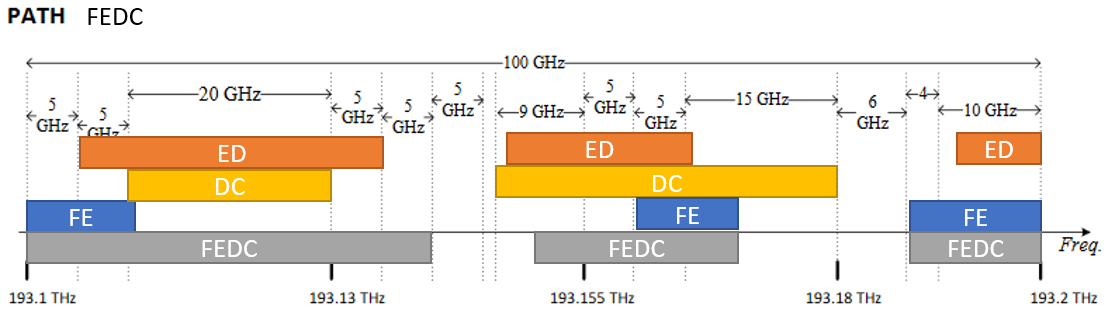
\includegraphics[scale=0.5]{spectrum-path-fedc}
    \caption{Path FEDC spectrum usage}
    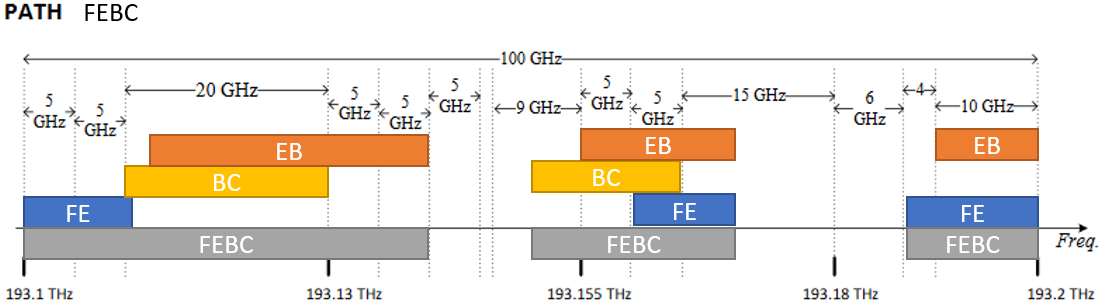
\includegraphics[scale=0.5]{spectrum-path-febc}
    \caption{Path FEBC spectrum usage}
    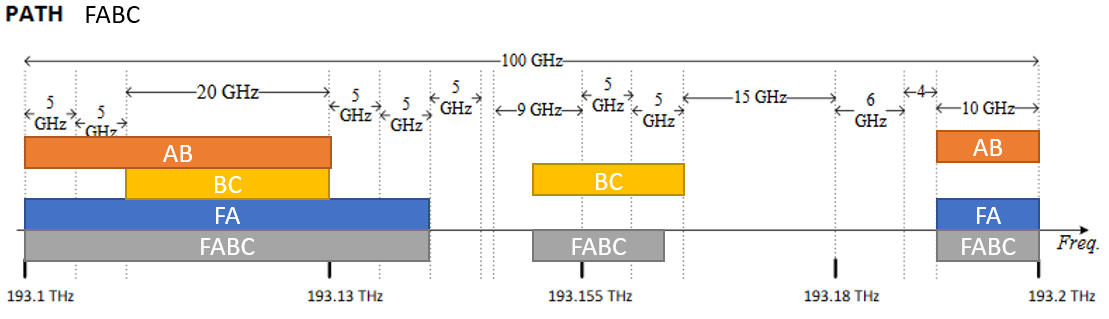
\includegraphics[scale=0.5]{spectrum-path-fabc}
    \caption{Path FABC spectrum usage}
\end{figure}

\subsection{}
\subsubsection{Maximum Transparent Reach}

The maximum transparent reach is 93.96 km.

\subsubsection{Different paths from $B \to D$}
\begin{table}[htb!]
    \centering
    \begin{tabular}{|c|c|c|}
    \hline
         Path & Distance & Is it achievable \\ \hline
         BCD & 50 Km & Yes \\ \hline
         BED & 40 Km & Yes \\ \hline
         BAFED & 85 Km & Yes\\ \hline

    \end{tabular}
    \caption{Results for 70 Gb/s}
\end{table}

\subsubsection{Sketch of the Available spectrum for each Achievable Routing Path}


\begin{figure}[htb!]
    \centering
    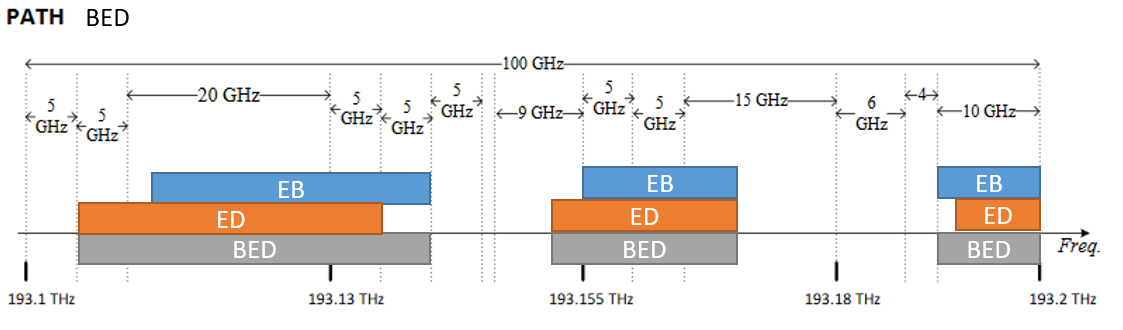
\includegraphics[scale=0.5]{spectrum-path-bed}
    \caption{Path BED spectrum usage}
    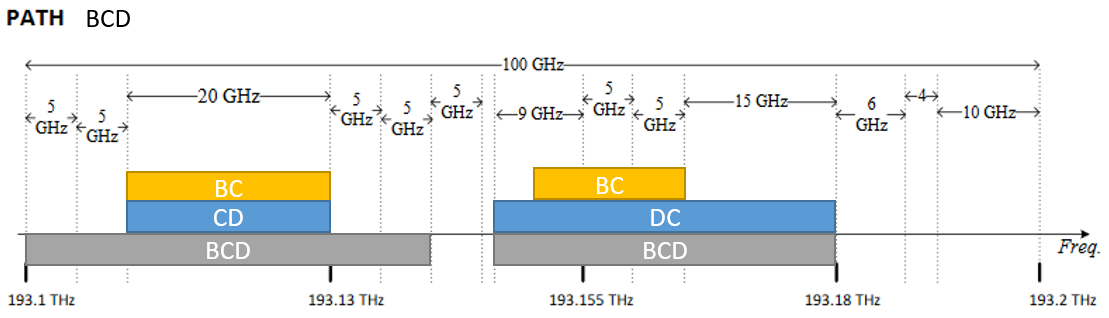
\includegraphics[scale=0.5]{spectrum-path-bcd}
    \caption{Path BCD spectrum usage}
    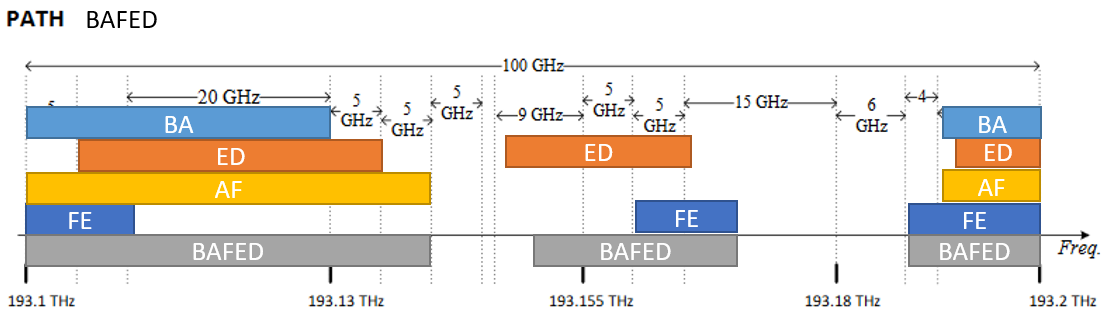
\includegraphics[scale=0.5]{spectrum-path-bafed}
    \caption{Path BAFED spectrum usage}
\end{figure}

\subsection{}
\subsubsection{Maximum Transparent Reach}

The maximum transparent reach is 86.68 km.

\subsubsection{Different paths from $A \to E$}
You can see the different paths available from A to E in Table 9.

\begin{table}[htb!]
    \centering
    \begin{tabular}{|c|c|c|}
    \hline
         Path & Distance & Is it achievable \\ \hline
         AFE & 45 Km & Yes \\ \hline
         ABE & 40 Km & Yes \\ \hline
         ABCDE & 90 Km & No\\ \hline

    \end{tabular}
    \caption{Results for 90 Gb/s}
\end{table}

\subsubsection{Sketch of the Available spectrum for each Achievable Routing Path}
You can see the sketches in Figure 8 to 9.

\begin{figure}[htb!]
    \centering
    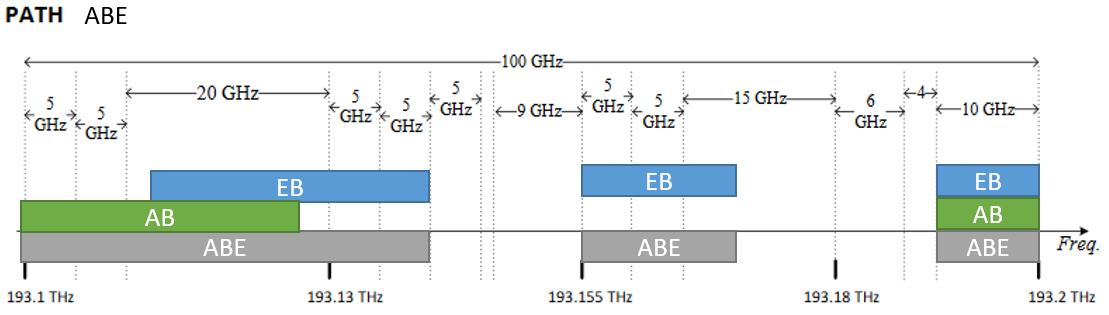
\includegraphics[scale=0.5]{spectrum-path-abe}
    \caption{Path ABE spectrum usage}
    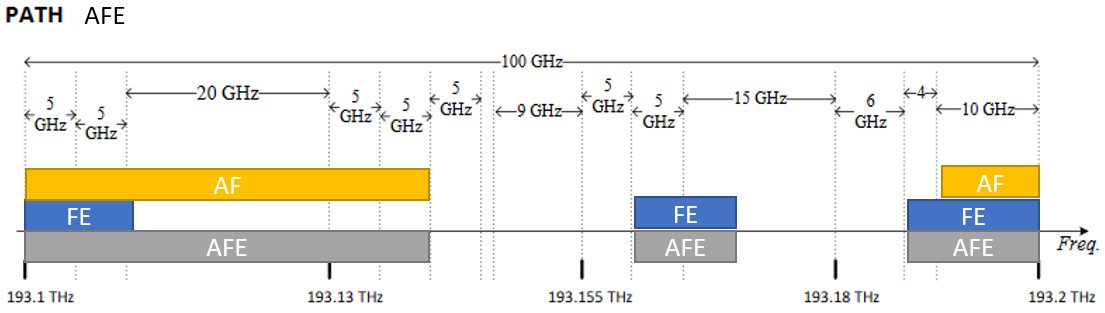
\includegraphics[scale=0.5]{spectrum-path-afe}
    \caption{Path AFE spectrum usage}
\end{figure}

\section{Identifying achievable routing paths by spectrum}
\setcounter{subsection}{4}
\subsection{Routing Table result}
You can find the routing table in table 10.

\subsection{Sketch of the Spectrum Occupancy}

You can find the sketch of the spectrum occupancy in figure 9.

\begin{table}[htb!]
    \centering
    \begin{tabular}{|c|c|c|p{2.5cm}|c|c|p{2.5cm}|}
    \hline
        Node & Path & Laser Frequency & OFDM or Nyquist & Baud Rate & QAM level & If OFDM, occupied bandwidths \\ \hline
        F & FABC & 193.19 THz & Nyquist & 11 & 64 & -  \\ \hline
        B & BED & 193.18 THz & Nyquist & 15.40 & 64 & - \\ \hline
        A & AFE & 193.16 THz & OFDM & 29.13 & 16 & 193.14 to 193.16 | 193.17 to 193.18 \\ \hline
    \end{tabular}
    \caption{Routing Decision Table}
\end{table}

\begin{figure}[htb!]
    \centering
    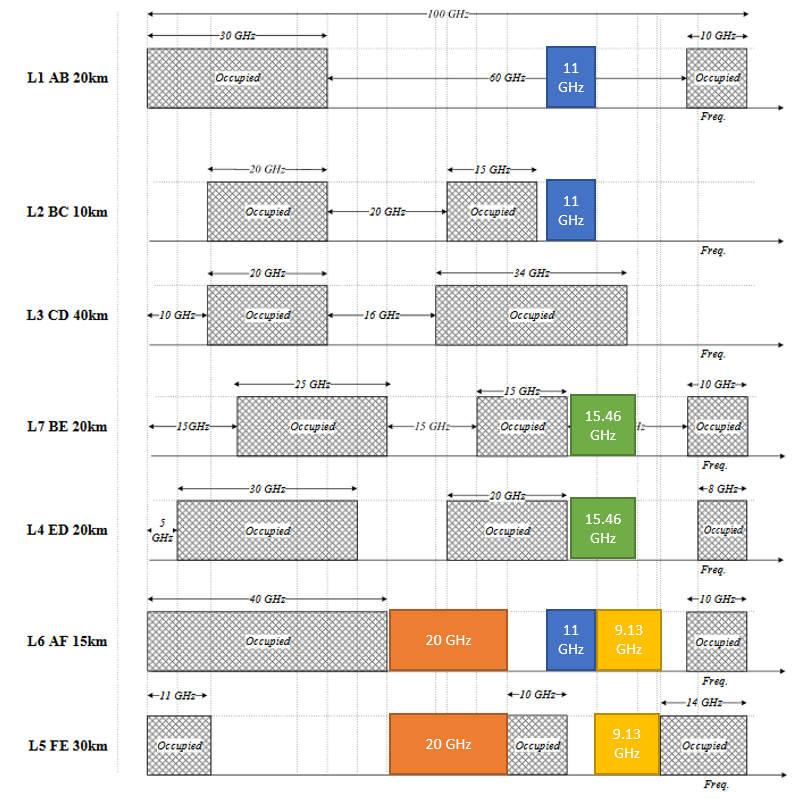
\includegraphics[scale=0.5]{route-allocation}
    \caption{Route Allocation}
\end{figure}

\subsection{}

In this subsection, I will first discuss the trade-offs between the options mentioned and later I will explain how these options affected our routing table choice.

\subsubsection{OFDM vs. Nyquist}
OFDM provides better flexibility compared to the Nyquist at the cost of requiring more bandwidth.

\subsubsection{7\% vs 20\%}
FEC equal to the value of 7\% provides lower $R_b$ while requiring less bandwidth compared to the 20\% FEC. Also, 20\% FEC provides better system reach compared to the FEC 7\%.

\subsubsection{QAM Levels}
As the modulation becomes more advanced, the system reach decreases. On the other hand, spectral efficiency increases. So the trade-off in choosing different QAM levels is between system reach and spectral efficiency.

Now that we have discussed different trade-offs in choosing different parameters I will explain the routing decisions that were made in creating the routing decision table. First, we will choose the shortest path among all different paths. Because, this will give us more choices in choosing different options available for different paths. So the paths chosen are as follows:

\begin{itemize}
    \item $F \to A \to B \to C$
    
    In this path we have about 25 GHz continuous bandwidth available. Also, we should ensure that the options chosen for the routing path should provide at least 50 Gb/s. Additionally, we should ensure that at least 45 Km system reach is available. From the options available, I have chosen the one with the least amount of spectral usage. This is to ensure that we are using the least amount of bandwidth. The choice that I have made is described in table 10.
    
    \item $B \to E \to D$
    
    In this path we have about 20 GHz of continuous bandwidth available. Also, we should ensure that the options chosen for the routing path should provide at least 70 Gb/s. Additionally, we should ensure that at least 40 Km system reach is available.  From the options available, I have chosen the one with the least amount of spectral usage. This is to ensure that we are using the least amount of bandwidth. The choice that I have made is described in table 10.
    
    \item $A \to F \to E$
    
    In this path we have about 20 GHz of continuous bandwidth available. Also, we should ensure that the options chosen for the routing path should provide at least 90 Gb/s. Additionally, we should ensure that at least 45 Km system reach is available. One thing to notice in this path, is that we have to have choose the longer path in this case. Because, the other path conflicts with the frequency used by other paths used by previous sections. Also, in this section we were not able to to choose the option with the least amount of bandwidth usage. So, in this case we had to go with the OFDM that provides the option of using non continuous bandwidths. The choice that I have made is described in table 10.
    
\end{itemize}

\end{document}
